\documentclass[1p]{elsarticle_modified}
%\bibliographystyle{elsarticle-num}

%\usepackage[colorlinks]{hyperref}
%\usepackage{abbrmath_seonhwa} %\Abb, \Ascr, \Acal ,\Abf, \Afrak
\usepackage{amsfonts}
\usepackage{amssymb}
\usepackage{amsmath}
\usepackage{amsthm}
\usepackage{scalefnt}
\usepackage{amsbsy}
\usepackage{kotex}
\usepackage{caption}
\usepackage{subfig}
\usepackage{color}
\usepackage{graphicx}
\usepackage{xcolor} %% white, black, red, green, blue, cyan, magenta, yellow
\usepackage{float}
\usepackage{setspace}
\usepackage{hyperref}

\usepackage{tikz}
\usetikzlibrary{arrows}

\usepackage{multirow}
\usepackage{array} % fixed length table
\usepackage{hhline}

%%%%%%%%%%%%%%%%%%%%%
\makeatletter
\renewcommand*\env@matrix[1][\arraystretch]{%
	\edef\arraystretch{#1}%
	\hskip -\arraycolsep
	\let\@ifnextchar\new@ifnextchar
	\array{*\c@MaxMatrixCols c}}
\makeatother %https://tex.stackexchange.com/questions/14071/how-can-i-increase-the-line-spacing-in-a-matrix
%%%%%%%%%%%%%%%

\usepackage[normalem]{ulem}

\newcommand{\msout}[1]{\ifmmode\text{\sout{\ensuremath{#1}}}\else\sout{#1}\fi}
%SOURCE: \msout is \stkout macro in https://tex.stackexchange.com/questions/20609/strikeout-in-math-mode

\newcommand{\cancel}[1]{
	\ifmmode
	{\color{red}\msout{#1}}
	\else
	{\color{red}\sout{#1}}
	\fi
}

\newcommand{\add}[1]{
	{\color{blue}\uwave{#1}}
}

\newcommand{\replace}[2]{
	\ifmmode
	{\color{red}\msout{#1}}{\color{blue}\uwave{#2}}
	\else
	{\color{red}\sout{#1}}{\color{blue}\uwave{#2}}
	\fi
}

\newcommand{\Sol}{\mathcal{S}} %segment
\newcommand{\D}{D} %diagram
\newcommand{\A}{\mathcal{A}} %arc


%%%%%%%%%%%%%%%%%%%%%%%%%%%%%5 test

\def\sl{\operatorname{\textup{SL}}(2,\Cbb)}
\def\psl{\operatorname{\textup{PSL}}(2,\Cbb)}
\def\quan{\mkern 1mu \triangleright \mkern 1mu}

\theoremstyle{definition}
\newtheorem{thm}{Theorem}[section]
\newtheorem{prop}[thm]{Proposition}
\newtheorem{lem}[thm]{Lemma}
\newtheorem{ques}[thm]{Question}
\newtheorem{cor}[thm]{Corollary}
\newtheorem{defn}[thm]{Definition}
\newtheorem{exam}[thm]{Example}
\newtheorem{rmk}[thm]{Remark}
\newtheorem{alg}[thm]{Algorithm}

\newcommand{\I}{\sqrt{-1}}
\begin{document}

%\begin{frontmatter}
%
%\title{Boundary parabolic representations of knots up to 8 crossings}
%
%%% Group authors per affiliation:
%\author{Yunhi Cho} 
%\address{Department of Mathematics, University of Seoul, Seoul, Korea}
%\ead{yhcho@uos.ac.kr}
%
%
%\author{Seonhwa Kim} %\fnref{s_kim}}
%\address{Center for Geometry and Physics, Institute for Basic Science, Pohang, 37673, Korea}
%\ead{ryeona17@ibs.re.kr}
%
%\author{Hyuk Kim}
%\address{Department of Mathematical Sciences, Seoul National University, Seoul 08826, Korea}
%\ead{hyukkim@snu.ac.kr}
%
%\author{Seokbeom Yoon}
%\address{Department of Mathematical Sciences, Seoul National University, Seoul, 08826,  Korea}
%\ead{sbyoon15@snu.ac.kr}
%
%\begin{abstract}
%We find all boundary parabolic representation of knots up to 8 crossings.
%
%\end{abstract}
%\begin{keyword}
%    \MSC[2010] 57M25 
%\end{keyword}
%
%\end{frontmatter}

%\linenumbers
%\tableofcontents
%
\newcommand\colored[1]{\textcolor{white}{\rule[-0.35ex]{0.8em}{1.4ex}}\kern-0.8em\color{red} #1}%
%\newcommand\colored[1]{\textcolor{white}{ #1}\kern-2.17ex	\textcolor{white}{ #1}\kern-1.81ex	\textcolor{white}{ #1}\kern-2.15ex\color{red}#1	}

{\Large $\underline{12a_{0942}~(K12a_{0942})}$}

\setlength{\tabcolsep}{10pt}
\renewcommand{\arraystretch}{1.6}
\vspace{1cm}\begin{tabular}{m{100pt}>{\centering\arraybackslash}m{274pt}}
\multirow{5}{120pt}{
	\centering
	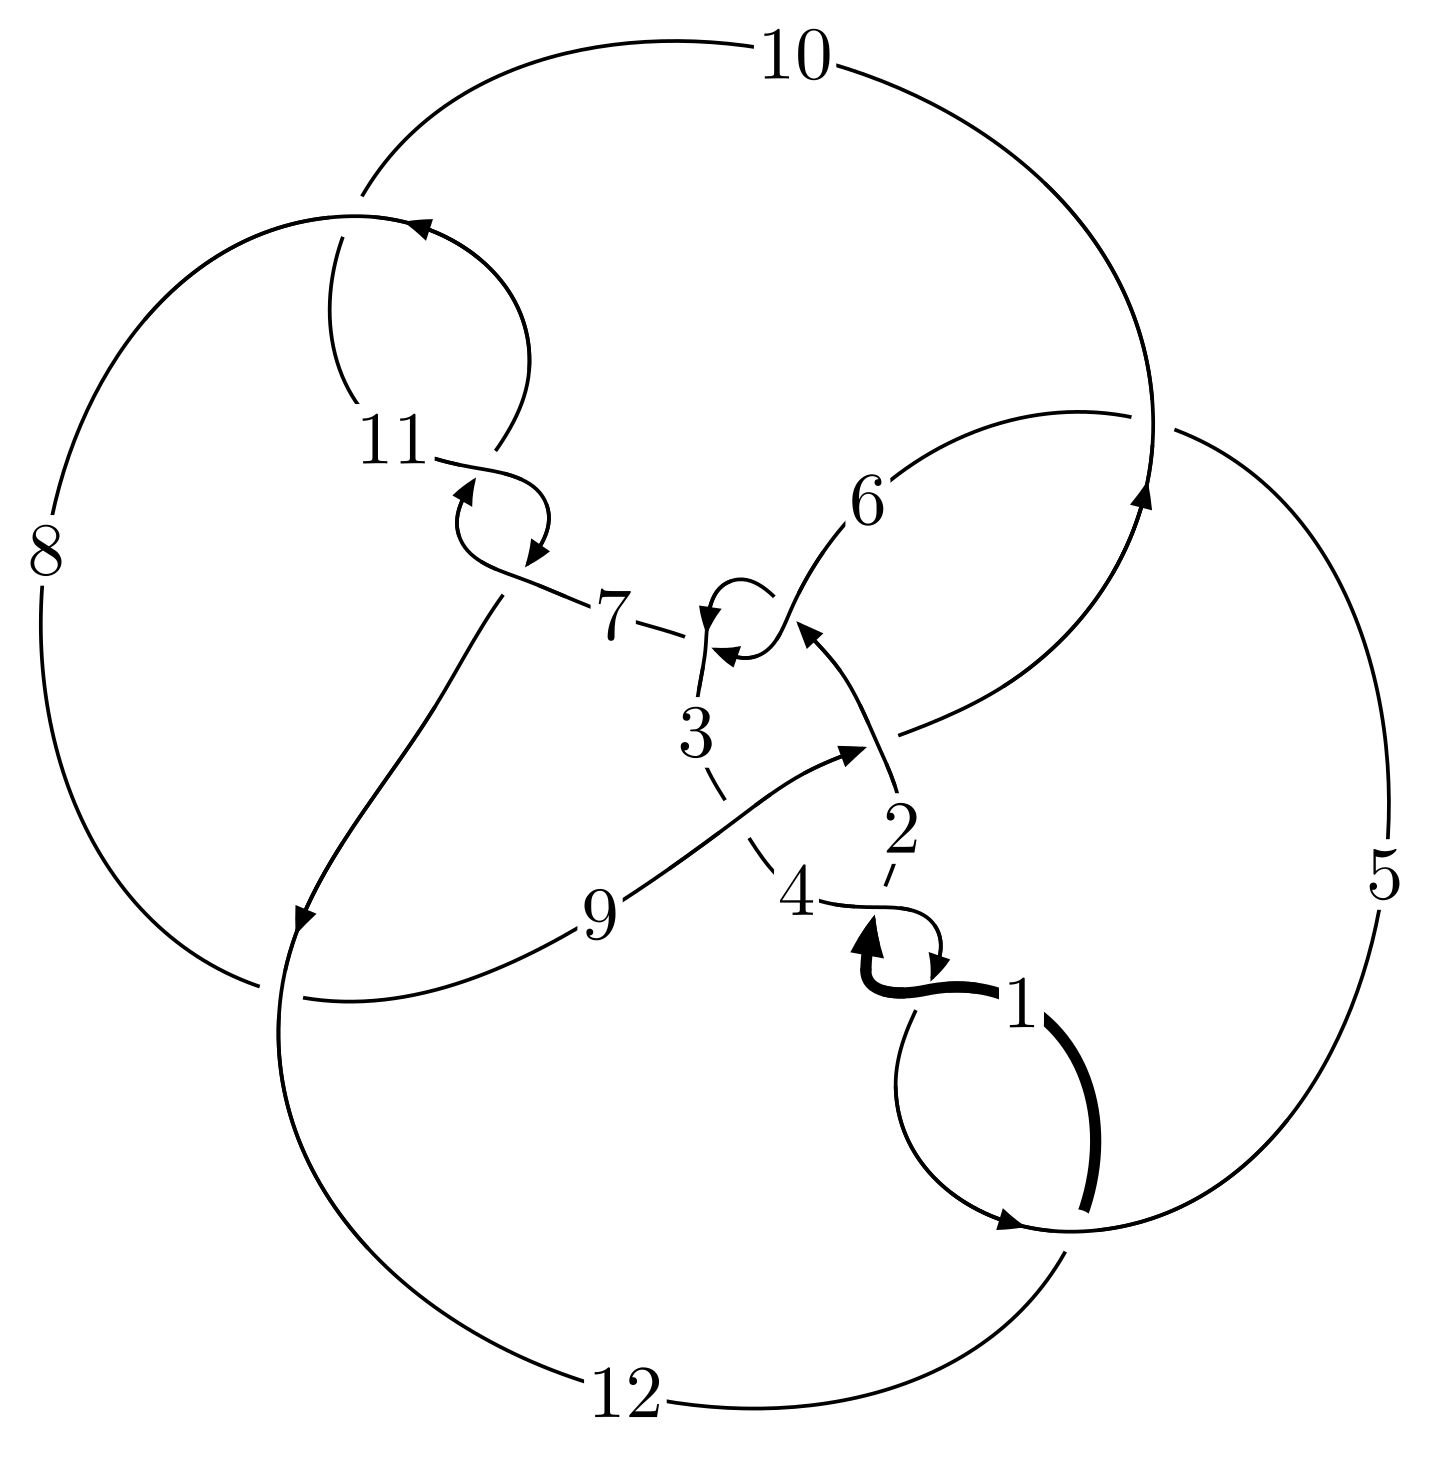
\includegraphics[width=112pt]{../../../GIT/diagram.site/Diagrams/png/1743_12a_0942.png}\\
\ \ \ A knot diagram\footnotemark}&
\allowdisplaybreaks
\textbf{Linearized knot diagam} \\
\cline{2-2}
 &
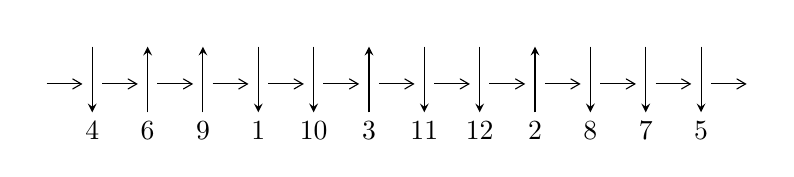
\begin{tikzpicture}[x=20pt, y=17pt]
	% nodes
	\node (C0) at (0, 0) {};
	\node (C1) at (1, 0) {};
	\node (C1U) at (1, +1) {};
	\node (C1D) at (1, -1) {4};

	\node (C2) at (2, 0) {};
	\node (C2U) at (2, +1) {};
	\node (C2D) at (2, -1) {6};

	\node (C3) at (3, 0) {};
	\node (C3U) at (3, +1) {};
	\node (C3D) at (3, -1) {9};

	\node (C4) at (4, 0) {};
	\node (C4U) at (4, +1) {};
	\node (C4D) at (4, -1) {1};

	\node (C5) at (5, 0) {};
	\node (C5U) at (5, +1) {};
	\node (C5D) at (5, -1) {10};

	\node (C6) at (6, 0) {};
	\node (C6U) at (6, +1) {};
	\node (C6D) at (6, -1) {3};

	\node (C7) at (7, 0) {};
	\node (C7U) at (7, +1) {};
	\node (C7D) at (7, -1) {11};

	\node (C8) at (8, 0) {};
	\node (C8U) at (8, +1) {};
	\node (C8D) at (8, -1) {12};

	\node (C9) at (9, 0) {};
	\node (C9U) at (9, +1) {};
	\node (C9D) at (9, -1) {2};

	\node (C10) at (10, 0) {};
	\node (C10U) at (10, +1) {};
	\node (C10D) at (10, -1) {8};

	\node (C11) at (11, 0) {};
	\node (C11U) at (11, +1) {};
	\node (C11D) at (11, -1) {7};

	\node (C12) at (12, 0) {};
	\node (C12U) at (12, +1) {};
	\node (C12D) at (12, -1) {5};
	\node (C13) at (13, 0) {};

	% arrows
	\draw[->,>={angle 60}]
	(C0) edge (C1) (C1) edge (C2) (C2) edge (C3) (C3) edge (C4) (C4) edge (C5) (C5) edge (C6) (C6) edge (C7) (C7) edge (C8) (C8) edge (C9) (C9) edge (C10) (C10) edge (C11) (C11) edge (C12) (C12) edge (C13) ;	\draw[->,>=stealth]
	(C1U) edge (C1D) (C2D) edge (C2U) (C3D) edge (C3U) (C4U) edge (C4D) (C5U) edge (C5D) (C6D) edge (C6U) (C7U) edge (C7D) (C8U) edge (C8D) (C9D) edge (C9U) (C10U) edge (C10D) (C11U) edge (C11D) (C12U) edge (C12D) ;
	\end{tikzpicture} \\
\hhline{~~} \\& 
\textbf{Solving Sequence} \\ \cline{2-2} 
 &
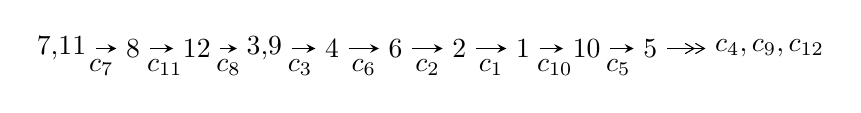
\begin{tikzpicture}[x=23pt, y=7pt]
	% node
	\node (A0) at (-1/8, 0) {7,11};
	\node (A1) at (1, 0) {8};
	\node (A2) at (2, 0) {12};
	\node (A3) at (49/16, 0) {3,9};
	\node (A4) at (33/8, 0) {4};
	\node (A5) at (41/8, 0) {6};
	\node (A6) at (49/8, 0) {2};
	\node (A7) at (57/8, 0) {1};
	\node (A8) at (65/8, 0) {10};
	\node (A9) at (73/8, 0) {5};
	\node (C1) at (1/2, -1) {$c_{7}$};
	\node (C2) at (3/2, -1) {$c_{11}$};
	\node (C3) at (5/2, -1) {$c_{8}$};
	\node (C4) at (29/8, -1) {$c_{3}$};
	\node (C5) at (37/8, -1) {$c_{6}$};
	\node (C6) at (45/8, -1) {$c_{2}$};
	\node (C7) at (53/8, -1) {$c_{1}$};
	\node (C8) at (61/8, -1) {$c_{10}$};
	\node (C9) at (69/8, -1) {$c_{5}$};
	\node (A10) at (11, 0) {$c_{4},c_{9},c_{12}$};

	% edge
	\draw[->,>=stealth]	
	(A0) edge (A1) (A1) edge (A2) (A2) edge (A3) (A3) edge (A4) (A4) edge (A5) (A5) edge (A6) (A6) edge (A7) (A7) edge (A8) (A8) edge (A9) ;
	\draw[->>,>={angle 60}]	
	(A9) edge (A10);
\end{tikzpicture} \\ 

\end{tabular} \\

\footnotetext{
The image of knot diagram is generated by the software ``\textbf{Draw programme}" developed by Andrew Bartholomew(\url{http://www.layer8.co.uk/maths/draw/index.htm\#Running-draw}), where we modified some parts for our purpose(\url{https://github.com/CATsTAILs/LinksPainter}).
}\phantom \\ \newline 
\centering \textbf{Ideals for irreducible components\footnotemark of $X_{\text{par}}$} 
 
\begin{align*}
I^u_{1}&=\langle 
-6.67572\times10^{88} u^{91}+2.35834\times10^{89} u^{90}+\cdots+2.42279\times10^{90} b+9.70979\times10^{89},\\
\phantom{I^u_{1}}&\phantom{= \langle  }1.80595\times10^{90} u^{91}+3.65341\times10^{90} u^{90}+\cdots+2.18051\times10^{91} a+1.03035\times10^{91},\;u^{92}+3 u^{91}+\cdots+49 u+9\rangle \\
I^u_{2}&=\langle 
-9 u^2 a-18 a u-3 u^2+23 b-3 a-6 u-1,\;-3 u^2 a+3 a^2+3 a u+3 u^2-3 a+4,\;u^3- u^2+2 u-1\rangle \\
\\
\end{align*}
\raggedright * 2 irreducible components of $\dim_{\mathbb{C}}=0$, with total 98 representations.\\
\footnotetext{All coefficients of polynomials are rational numbers. But the coefficients are sometimes approximated in decimal forms when there is not enough margin.}
\newpage
\renewcommand{\arraystretch}{1}
\centering \section*{I. $I^u_{1}= \langle -6.68\times10^{88} u^{91}+2.36\times10^{89} u^{90}+\cdots+2.42\times10^{90} b+9.71\times10^{89},\;1.81\times10^{90} u^{91}+3.65\times10^{90} u^{90}+\cdots+2.18\times10^{91} a+1.03\times10^{91},\;u^{92}+3 u^{91}+\cdots+49 u+9 \rangle$}
\flushleft \textbf{(i) Arc colorings}\\
\begin{tabular}{m{7pt} m{180pt} m{7pt} m{180pt} }
\flushright $a_{7}=$&$\begin{pmatrix}1\\0\end{pmatrix}$ \\
\flushright $a_{11}=$&$\begin{pmatrix}0\\u\end{pmatrix}$ \\
\flushright $a_{8}=$&$\begin{pmatrix}1\\u^2\end{pmatrix}$ \\
\flushright $a_{12}=$&$\begin{pmatrix}- u\\u\end{pmatrix}$ \\
\flushright $a_{3}=$&$\begin{pmatrix}-0.0828225 u^{91}-0.167548 u^{90}+\cdots-3.52927 u-0.472529\\0.0275538 u^{91}-0.0973397 u^{90}+\cdots-1.86772 u-0.400769\end{pmatrix}$ \\
\flushright $a_{9}=$&$\begin{pmatrix}- u^4- u^2+1\\u^4+2 u^2\end{pmatrix}$ \\
\flushright $a_{4}=$&$\begin{pmatrix}0.0509100 u^{91}+0.622642 u^{90}+\cdots+12.8628 u+2.47080\\-0.324534 u^{91}-1.12865 u^{90}+\cdots-16.5700 u-3.59604\end{pmatrix}$ \\
\flushright $a_{6}=$&$\begin{pmatrix}0.000609590 u^{91}+0.892534 u^{90}+\cdots-5.59951 u-1.33977\\-1.01318 u^{91}-2.80973 u^{90}+\cdots-41.4443 u-9.83553\end{pmatrix}$ \\
\flushright $a_{2}=$&$\begin{pmatrix}-0.210669 u^{91}-0.186692 u^{90}+\cdots-7.66553 u-4.08858\\-0.171606 u^{91}-0.788526 u^{90}+\cdots-11.2024 u-3.44047\end{pmatrix}$ \\
\flushright $a_{1}=$&$\begin{pmatrix}0.0567726 u^{91}+0.233111 u^{90}+\cdots+5.88148 u+1.02278\\0.283527 u^{91}+0.499883 u^{90}+\cdots+13.4607 u+2.66381\end{pmatrix}$ \\
\flushright $a_{10}=$&$\begin{pmatrix}u\\u^3+u\end{pmatrix}$ \\
\flushright $a_{5}=$&$\begin{pmatrix}-0.161712 u^{91}+0.315650 u^{90}+\cdots-3.68445 u-0.838694\\-0.539534 u^{91}-1.79824 u^{90}+\cdots-33.6623 u-8.52519\end{pmatrix}$\\&\end{tabular}
\flushleft \textbf{(ii) Obstruction class $= -1$}\\~\\
\flushleft \textbf{(iii) Cusp Shapes $= -0.692795 u^{91}-2.25332 u^{90}+\cdots-40.8738 u-9.09423$}\\~\\
\newpage\renewcommand{\arraystretch}{1}
\flushleft \textbf{(iv) u-Polynomials at the component}\newline \\
\begin{tabular}{m{50pt}|m{274pt}}
Crossings & \hspace{64pt}u-Polynomials at each crossing \\
\hline $$\begin{aligned}c_{1},c_{4},c_{12}\end{aligned}$$&$\begin{aligned}
&u^{92}-4 u^{91}+\cdots-4 u+1
\end{aligned}$\\
\hline $$\begin{aligned}c_{2},c_{6}\end{aligned}$$&$\begin{aligned}
&u^{92}-4 u^{91}+\cdots-4 u+1
\end{aligned}$\\
\hline $$\begin{aligned}c_{3}\end{aligned}$$&$\begin{aligned}
&27(27 u^{92}-27 u^{91}+\cdots+133643 u-6581)
\end{aligned}$\\
\hline $$\begin{aligned}c_{5}\end{aligned}$$&$\begin{aligned}
&27(27 u^{92}-54 u^{91}+\cdots+1430027 u+751139)
\end{aligned}$\\
\hline $$\begin{aligned}c_{7},c_{10},c_{11}\end{aligned}$$&$\begin{aligned}
&u^{92}-3 u^{91}+\cdots-49 u+9
\end{aligned}$\\
\hline $$\begin{aligned}c_{8}\end{aligned}$$&$\begin{aligned}
&u^{92}+3 u^{91}+\cdots+30601 u+21969
\end{aligned}$\\
\hline $$\begin{aligned}c_{9}\end{aligned}$$&$\begin{aligned}
&u^{92}+3 u^{91}+\cdots+4320 u+5184
\end{aligned}$\\
\hline
\end{tabular}\\~\\
\newpage\renewcommand{\arraystretch}{1}
\flushleft \textbf{(v) Riley Polynomials at the component}\newline \\
\begin{tabular}{m{50pt}|m{274pt}}
Crossings & \hspace{64pt}Riley Polynomials at each crossing \\
\hline $$\begin{aligned}c_{1},c_{4},c_{12}\end{aligned}$$&$\begin{aligned}
&y^{92}+88 y^{91}+\cdots-10 y+1
\end{aligned}$\\
\hline $$\begin{aligned}c_{2},c_{6}\end{aligned}$$&$\begin{aligned}
&y^{92}-52 y^{91}+\cdots-10 y+1
\end{aligned}$\\
\hline $$\begin{aligned}c_{3}\end{aligned}$$&$\begin{aligned}
&729(729 y^{92}-38313 y^{91}+\cdots-6.42023\times10^{9} y+4.33096\times10^{7})
\end{aligned}$\\
\hline $$\begin{aligned}c_{5}\end{aligned}$$&$\begin{aligned}
&729\\
&\cdot(729 y^{92}+16362 y^{91}+\cdots+15225683884841 y+564209797321)
\end{aligned}$\\
\hline $$\begin{aligned}c_{7},c_{10},c_{11}\end{aligned}$$&$\begin{aligned}
&y^{92}+83 y^{91}+\cdots-169 y+81
\end{aligned}$\\
\hline $$\begin{aligned}c_{8}\end{aligned}$$&$\begin{aligned}
&y^{92}- y^{91}+\cdots+12026870567 y+482636961
\end{aligned}$\\
\hline $$\begin{aligned}c_{9}\end{aligned}$$&$\begin{aligned}
&y^{92}-35 y^{91}+\cdots-347120640 y+26873856
\end{aligned}$\\
\hline
\end{tabular}\\~\\
\newpage\flushleft \textbf{(vi) Complex Volumes and Cusp Shapes}
$$\begin{array}{c|c|c}  
\text{Solutions to }I^u_{1}& \I (\text{vol} + \sqrt{-1}CS) & \text{Cusp shape}\\
 \hline 
\begin{aligned}
u &= -0.582390 + 0.791689 I \\
a &= \phantom{-}0.753577 - 0.347209 I \\
b &= -1.251090 + 0.475634 I\end{aligned}
 & \phantom{-}9.25726 - 8.18208 I & \phantom{-0.000000 } 0 \\ \hline\begin{aligned}
u &= -0.582390 - 0.791689 I \\
a &= \phantom{-}0.753577 + 0.347209 I \\
b &= -1.251090 - 0.475634 I\end{aligned}
 & \phantom{-}9.25726 + 8.18208 I & \phantom{-0.000000 } 0 \\ \hline\begin{aligned}
u &= \phantom{-}0.736262 + 0.628121 I \\
a &= \phantom{-}1.049820 + 0.457055 I \\
b &= -0.887252 + 0.284095 I\end{aligned}
 & \phantom{-}3.94303 - 3.83126 I & \phantom{-0.000000 } 0 \\ \hline\begin{aligned}
u &= \phantom{-}0.736262 - 0.628121 I \\
a &= \phantom{-}1.049820 - 0.457055 I \\
b &= -0.887252 - 0.284095 I\end{aligned}
 & \phantom{-}3.94303 + 3.83126 I & \phantom{-0.000000 } 0 \\ \hline\begin{aligned}
u &= \phantom{-}0.926342 + 0.164936 I \\
a &= \phantom{-}0.460377 + 0.377356 I \\
b &= -0.729328 + 0.179095 I\end{aligned}
 & \phantom{-}2.52480 - 1.25642 I & \phantom{-0.000000 } 0 \\ \hline\begin{aligned}
u &= \phantom{-}0.926342 - 0.164936 I \\
a &= \phantom{-}0.460377 - 0.377356 I \\
b &= -0.729328 - 0.179095 I\end{aligned}
 & \phantom{-}2.52480 + 1.25642 I & \phantom{-0.000000 } 0 \\ \hline\begin{aligned}
u &= \phantom{-}0.323996 + 1.013050 I \\
a &= \phantom{-}0.630042 - 0.069778 I \\
b &= -0.265885 - 0.472333 I\end{aligned}
 & \phantom{-}5.03694 - 3.16909 I & \phantom{-0.000000 } 0 \\ \hline\begin{aligned}
u &= \phantom{-}0.323996 - 1.013050 I \\
a &= \phantom{-}0.630042 + 0.069778 I \\
b &= -0.265885 + 0.472333 I\end{aligned}
 & \phantom{-}5.03694 + 3.16909 I & \phantom{-0.000000 } 0 \\ \hline\begin{aligned}
u &= -0.094010 + 1.097530 I \\
a &= -1.038130 + 0.233071 I \\
b &= \phantom{-}0.418611 + 0.766435 I\end{aligned}
 & \phantom{-}0.233678 - 0.500797 I & \phantom{-0.000000 } 0 \\ \hline\begin{aligned}
u &= -0.094010 - 1.097530 I \\
a &= -1.038130 - 0.233071 I \\
b &= \phantom{-}0.418611 - 0.766435 I\end{aligned}
 & \phantom{-}0.233678 + 0.500797 I & \phantom{-0.000000 } 0\\
 \hline 
 \end{array}$$\newpage$$\begin{array}{c|c|c}  
\text{Solutions to }I^u_{1}& \I (\text{vol} + \sqrt{-1}CS) & \text{Cusp shape}\\
 \hline 
\begin{aligned}
u &= -0.818478 + 0.331482 I \\
a &= \phantom{-}0.76020 - 1.33742 I \\
b &= -1.295560 - 0.541975 I\end{aligned}
 & \phantom{-}7.8020 + 13.0110 I & \phantom{-0.000000 } 0. - 8.15881 I \\ \hline\begin{aligned}
u &= -0.818478 - 0.331482 I \\
a &= \phantom{-}0.76020 + 1.33742 I \\
b &= -1.295560 + 0.541975 I\end{aligned}
 & \phantom{-}7.8020 - 13.0110 I & \phantom{-0.000000 -}0. + 8.15881 I \\ \hline\begin{aligned}
u &= -0.437432 + 0.765002 I \\
a &= -0.719368 + 0.448533 I \\
b &= \phantom{-}1.213080 - 0.455397 I\end{aligned}
 & \phantom{-}2.95349 - 4.88268 I & -4.00000 + 4.50142 I \\ \hline\begin{aligned}
u &= -0.437432 - 0.765002 I \\
a &= -0.719368 - 0.448533 I \\
b &= \phantom{-}1.213080 + 0.455397 I\end{aligned}
 & \phantom{-}2.95349 + 4.88268 I & -4.00000 - 4.50142 I \\ \hline\begin{aligned}
u &= \phantom{-}0.000013 + 1.147790 I \\
a &= \phantom{-}0.344767 - 0.348258 I \\
b &= -0.829604 + 0.540806 I\end{aligned}
 & \phantom{-}3.51439 - 1.54001 I & \phantom{-0.000000 } 0 \\ \hline\begin{aligned}
u &= \phantom{-}0.000013 - 1.147790 I \\
a &= \phantom{-}0.344767 + 0.348258 I \\
b &= -0.829604 - 0.540806 I\end{aligned}
 & \phantom{-}3.51439 + 1.54001 I & \phantom{-0.000000 } 0 \\ \hline\begin{aligned}
u &= \phantom{-}0.374112 + 1.092450 I \\
a &= -0.830199 - 0.416954 I \\
b &= \phantom{-}0.927867 - 0.309390 I\end{aligned}
 & \phantom{-}1.93950 - 4.31636 I & \phantom{-0.000000 } 0 \\ \hline\begin{aligned}
u &= \phantom{-}0.374112 - 1.092450 I \\
a &= -0.830199 + 0.416954 I \\
b &= \phantom{-}0.927867 + 0.309390 I\end{aligned}
 & \phantom{-}1.93950 + 4.31636 I & \phantom{-0.000000 } 0 \\ \hline\begin{aligned}
u &= -0.374410 + 0.730981 I \\
a &= \phantom{-}0.902557 - 0.188982 I \\
b &= -0.056183 - 0.815962 I\end{aligned}
 & \phantom{-}5.65365 - 3.41644 I & -0.205199 + 1.266815 I \\ \hline\begin{aligned}
u &= -0.374410 - 0.730981 I \\
a &= \phantom{-}0.902557 + 0.188982 I \\
b &= -0.056183 + 0.815962 I\end{aligned}
 & \phantom{-}5.65365 + 3.41644 I & -0.205199 - 1.266815 I\\
 \hline 
 \end{array}$$\newpage$$\begin{array}{c|c|c}  
\text{Solutions to }I^u_{1}& \I (\text{vol} + \sqrt{-1}CS) & \text{Cusp shape}\\
 \hline 
\begin{aligned}
u &= \phantom{-}0.819573\phantom{ +0.000000I} \\
a &= \phantom{-}0.0197403\phantom{ +0.000000I} \\
b &= \phantom{-}0.744911\phantom{ +0.000000I}\end{aligned}
 & -1.38150\phantom{ +0.000000I} & -13.5870\phantom{ +0.000000I} \\ \hline\begin{aligned}
u &= -0.760866 + 0.288446 I \\
a &= -0.62010 + 1.40146 I \\
b &= \phantom{-}1.286890 + 0.560835 I\end{aligned}
 & \phantom{-}1.36094 + 9.14769 I & -3.11665 - 8.62512 I \\ \hline\begin{aligned}
u &= -0.760866 - 0.288446 I \\
a &= -0.62010 - 1.40146 I \\
b &= \phantom{-}1.286890 - 0.560835 I\end{aligned}
 & \phantom{-}1.36094 - 9.14769 I & -3.11665 + 8.62512 I \\ \hline\begin{aligned}
u &= \phantom{-}0.756425 + 0.260905 I \\
a &= \phantom{-}0.485720 + 0.109400 I \\
b &= -0.302020 - 0.238032 I\end{aligned}
 & \phantom{-}2.69497 - 1.07990 I & -4.94046 + 1.01805 I \\ \hline\begin{aligned}
u &= \phantom{-}0.756425 - 0.260905 I \\
a &= \phantom{-}0.485720 - 0.109400 I \\
b &= -0.302020 + 0.238032 I\end{aligned}
 & \phantom{-}2.69497 + 1.07990 I & -4.94046 - 1.01805 I \\ \hline\begin{aligned}
u &= \phantom{-}0.703199 + 0.371330 I \\
a &= -0.929795 - 0.803087 I \\
b &= \phantom{-}0.871833 - 0.211011 I\end{aligned}
 & -0.61831 - 2.08055 I & -9.77125 + 9.25183 I \\ \hline\begin{aligned}
u &= \phantom{-}0.703199 - 0.371330 I \\
a &= -0.929795 + 0.803087 I \\
b &= \phantom{-}0.871833 + 0.211011 I\end{aligned}
 & -0.61831 + 2.08055 I & -9.77125 - 9.25183 I \\ \hline\begin{aligned}
u &= -0.736185 + 0.281983 I \\
a &= -0.479375 + 0.643889 I \\
b &= -0.102011 + 1.017520 I\end{aligned}
 & \phantom{-}4.08651 + 7.45020 I & -2.56752 - 6.27902 I \\ \hline\begin{aligned}
u &= -0.736185 - 0.281983 I \\
a &= -0.479375 - 0.643889 I \\
b &= -0.102011 - 1.017520 I\end{aligned}
 & \phantom{-}4.08651 - 7.45020 I & -2.56752 + 6.27902 I \\ \hline\begin{aligned}
u &= -0.142124 + 1.263210 I \\
a &= \phantom{-}1.52577 - 0.30777 I \\
b &= -0.745186 - 0.965258 I\end{aligned}
 & \phantom{-}2.80330 + 4.03627 I & \phantom{-0.000000 } 0\\
 \hline 
 \end{array}$$\newpage$$\begin{array}{c|c|c}  
\text{Solutions to }I^u_{1}& \I (\text{vol} + \sqrt{-1}CS) & \text{Cusp shape}\\
 \hline 
\begin{aligned}
u &= -0.142124 - 1.263210 I \\
a &= \phantom{-}1.52577 + 0.30777 I \\
b &= -0.745186 + 0.965258 I\end{aligned}
 & \phantom{-}2.80330 - 4.03627 I & \phantom{-0.000000 } 0 \\ \hline\begin{aligned}
u &= \phantom{-}0.164963 + 1.270790 I \\
a &= \phantom{-}0.050965 - 0.698499 I \\
b &= -0.577119 - 0.165305 I\end{aligned}
 & \phantom{-}3.85258 - 2.03665 I & \phantom{-0.000000 } 0 \\ \hline\begin{aligned}
u &= \phantom{-}0.164963 - 1.270790 I \\
a &= \phantom{-}0.050965 + 0.698499 I \\
b &= -0.577119 + 0.165305 I\end{aligned}
 & \phantom{-}3.85258 + 2.03665 I & \phantom{-0.000000 } 0 \\ \hline\begin{aligned}
u &= -0.656857 + 0.267157 I \\
a &= \phantom{-}0.44312 - 1.61945 I \\
b &= -1.248510 - 0.587775 I\end{aligned}
 & \phantom{-}1.84603 + 4.13199 I & -1.86475 - 5.14943 I \\ \hline\begin{aligned}
u &= -0.656857 - 0.267157 I \\
a &= \phantom{-}0.44312 + 1.61945 I \\
b &= -1.248510 + 0.587775 I\end{aligned}
 & \phantom{-}1.84603 - 4.13199 I & -1.86475 + 5.14943 I \\ \hline\begin{aligned}
u &= \phantom{-}0.128671 + 1.295620 I \\
a &= -3.84498 + 0.47312 I \\
b &= \phantom{-}1.203540 - 0.042147 I\end{aligned}
 & \phantom{-}9.63383 - 2.00341 I & \phantom{-0.000000 } 0 \\ \hline\begin{aligned}
u &= \phantom{-}0.128671 - 1.295620 I \\
a &= -3.84498 - 0.47312 I \\
b &= \phantom{-}1.203540 + 0.042147 I\end{aligned}
 & \phantom{-}9.63383 + 2.00341 I & \phantom{-0.000000 } 0 \\ \hline\begin{aligned}
u &= -0.581029 + 0.359352 I \\
a &= -0.222451 + 0.196065 I \\
b &= \phantom{-}1.348550 - 0.386647 I\end{aligned}
 & \phantom{-}8.85704 + 2.47164 I & \phantom{-}3.01205 - 4.35204 I \\ \hline\begin{aligned}
u &= -0.581029 - 0.359352 I \\
a &= -0.222451 - 0.196065 I \\
b &= \phantom{-}1.348550 + 0.386647 I\end{aligned}
 & \phantom{-}8.85704 - 2.47164 I & \phantom{-}3.01205 + 4.35204 I \\ \hline\begin{aligned}
u &= -0.642174 + 0.199804 I \\
a &= \phantom{-}0.535662 - 0.867543 I \\
b &= \phantom{-}0.182287 - 1.052460 I\end{aligned}
 & -2.15457 + 3.40976 I & -5.90227 - 8.24087 I\\
 \hline 
 \end{array}$$\newpage$$\begin{array}{c|c|c}  
\text{Solutions to }I^u_{1}& \I (\text{vol} + \sqrt{-1}CS) & \text{Cusp shape}\\
 \hline 
\begin{aligned}
u &= -0.642174 - 0.199804 I \\
a &= \phantom{-}0.535662 + 0.867543 I \\
b &= \phantom{-}0.182287 + 1.052460 I\end{aligned}
 & -2.15457 - 3.40976 I & -5.90227 + 8.24087 I \\ \hline\begin{aligned}
u &= \phantom{-}0.671704\phantom{ +0.000000I} \\
a &= -0.310781\phantom{ +0.000000I} \\
b &= \phantom{-}0.215837\phantom{ +0.000000I}\end{aligned}
 & -1.55032\phantom{ +0.000000I} & -7.74090\phantom{ +0.000000I} \\ \hline\begin{aligned}
u &= \phantom{-}0.259605 + 1.309660 I \\
a &= -0.247077 + 0.013717 I \\
b &= \phantom{-}0.097376 + 0.288479 I\end{aligned}
 & \phantom{-}2.60983 - 3.35368 I & \phantom{-0.000000 } 0 \\ \hline\begin{aligned}
u &= \phantom{-}0.259605 - 1.309660 I \\
a &= -0.247077 - 0.013717 I \\
b &= \phantom{-}0.097376 - 0.288479 I\end{aligned}
 & \phantom{-}2.60983 + 3.35368 I & \phantom{-0.000000 } 0 \\ \hline\begin{aligned}
u &= -0.516057 + 0.400667 I \\
a &= -0.76365 + 2.13859 I \\
b &= \phantom{-}1.185740 + 0.507231 I\end{aligned}
 & \phantom{-}9.09275 + 1.02296 I & \phantom{-}3.55453 - 4.18776 I \\ \hline\begin{aligned}
u &= -0.516057 - 0.400667 I \\
a &= -0.76365 - 2.13859 I \\
b &= \phantom{-}1.185740 - 0.507231 I\end{aligned}
 & \phantom{-}9.09275 - 1.02296 I & \phantom{-}3.55453 + 4.18776 I \\ \hline\begin{aligned}
u &= \phantom{-}0.503851 + 1.248960 I \\
a &= \phantom{-}1.103600 + 0.557191 I \\
b &= -0.967384 + 0.312417 I\end{aligned}
 & \phantom{-}6.83291 - 6.37350 I & \phantom{-0.000000 } 0 \\ \hline\begin{aligned}
u &= \phantom{-}0.503851 - 1.248960 I \\
a &= \phantom{-}1.103600 - 0.557191 I \\
b &= -0.967384 - 0.312417 I\end{aligned}
 & \phantom{-}6.83291 + 6.37350 I & \phantom{-0.000000 } 0 \\ \hline\begin{aligned}
u &= \phantom{-}0.163438 + 1.344350 I \\
a &= -0.54876 + 2.14293 I \\
b &= \phantom{-}0.884445 + 0.234151 I\end{aligned}
 & \phantom{-}10.19730 - 2.39866 I & \phantom{-0.000000 } 0 \\ \hline\begin{aligned}
u &= \phantom{-}0.163438 - 1.344350 I \\
a &= -0.54876 - 2.14293 I \\
b &= \phantom{-}0.884445 - 0.234151 I\end{aligned}
 & \phantom{-}10.19730 + 2.39866 I & \phantom{-0.000000 } 0\\
 \hline 
 \end{array}$$\newpage$$\begin{array}{c|c|c}  
\text{Solutions to }I^u_{1}& \I (\text{vol} + \sqrt{-1}CS) & \text{Cusp shape}\\
 \hline 
\begin{aligned}
u &= \phantom{-}0.223299 + 1.351700 I \\
a &= \phantom{-}2.70863 + 1.95015 I \\
b &= -1.068200 + 0.141951 I\end{aligned}
 & \phantom{-}5.06193 - 3.40170 I & \phantom{-0.000000 } 0 \\ \hline\begin{aligned}
u &= \phantom{-}0.223299 - 1.351700 I \\
a &= \phantom{-}2.70863 - 1.95015 I \\
b &= -1.068200 - 0.141951 I\end{aligned}
 & \phantom{-}5.06193 + 3.40170 I & \phantom{-0.000000 } 0 \\ \hline\begin{aligned}
u &= -0.188713 + 1.361780 I \\
a &= -0.486402 - 0.868672 I \\
b &= -0.389728 + 1.216040 I\end{aligned}
 & \phantom{-}3.87314 + 0.69064 I & \phantom{-0.000000 } 0 \\ \hline\begin{aligned}
u &= -0.188713 - 1.361780 I \\
a &= -0.486402 + 0.868672 I \\
b &= -0.389728 - 1.216040 I\end{aligned}
 & \phantom{-}3.87314 - 0.69064 I & \phantom{-0.000000 } 0 \\ \hline\begin{aligned}
u &= -0.251021 + 1.379070 I \\
a &= \phantom{-}0.729238 + 0.669618 I \\
b &= \phantom{-}0.135336 - 1.223050 I\end{aligned}
 & \phantom{-}2.87331 + 6.66260 I & \phantom{-0.000000 } 0 \\ \hline\begin{aligned}
u &= -0.251021 - 1.379070 I \\
a &= \phantom{-}0.729238 - 0.669618 I \\
b &= \phantom{-}0.135336 + 1.223050 I\end{aligned}
 & \phantom{-}2.87331 - 6.66260 I & \phantom{-0.000000 } 0 \\ \hline\begin{aligned}
u &= \phantom{-}0.574264 + 0.111966 I \\
a &= \phantom{-}0.22466 + 2.92931 I \\
b &= -0.931822 + 0.094872 I\end{aligned}
 & \phantom{-}0.395763 - 0.494287 I & \phantom{-}4.29552 - 12.70736 I \\ \hline\begin{aligned}
u &= \phantom{-}0.574264 - 0.111966 I \\
a &= \phantom{-}0.22466 - 2.92931 I \\
b &= -0.931822 - 0.094872 I\end{aligned}
 & \phantom{-}0.395763 + 0.494287 I & \phantom{-}4.29552 + 12.70736 I \\ \hline\begin{aligned}
u &= -0.14834 + 1.40864 I \\
a &= \phantom{-}2.08410 - 0.83521 I \\
b &= -1.48389 + 0.31155 I\end{aligned}
 & \phantom{-}8.76204 + 0.97088 I & \phantom{-0.000000 } 0 \\ \hline\begin{aligned}
u &= -0.14834 - 1.40864 I \\
a &= \phantom{-}2.08410 + 0.83521 I \\
b &= -1.48389 - 0.31155 I\end{aligned}
 & \phantom{-}8.76204 - 0.97088 I & \phantom{-0.000000 } 0\\
 \hline 
 \end{array}$$\newpage$$\begin{array}{c|c|c}  
\text{Solutions to }I^u_{1}& \I (\text{vol} + \sqrt{-1}CS) & \text{Cusp shape}\\
 \hline 
\begin{aligned}
u &= \phantom{-}0.28623 + 1.39773 I \\
a &= \phantom{-}0.315348 + 0.116776 I \\
b &= -0.023245 - 0.439811 I\end{aligned}
 & \phantom{-}7.95406 - 4.80757 I & \phantom{-0.000000 } 0 \\ \hline\begin{aligned}
u &= \phantom{-}0.28623 - 1.39773 I \\
a &= \phantom{-}0.315348 - 0.116776 I \\
b &= -0.023245 + 0.439811 I\end{aligned}
 & \phantom{-}7.95406 + 4.80757 I & \phantom{-0.000000 } 0 \\ \hline\begin{aligned}
u &= -0.25957 + 1.40499 I \\
a &= \phantom{-}2.14568 - 1.00660 I \\
b &= -1.35135 - 0.65463 I\end{aligned}
 & \phantom{-}7.18270 + 7.48451 I & \phantom{-0.000000 } 0 \\ \hline\begin{aligned}
u &= -0.25957 - 1.40499 I \\
a &= \phantom{-}2.14568 + 1.00660 I \\
b &= -1.35135 + 0.65463 I\end{aligned}
 & \phantom{-}7.18270 - 7.48451 I & \phantom{-0.000000 } 0 \\ \hline\begin{aligned}
u &= -0.08596 + 1.43421 I \\
a &= \phantom{-}0.312598 + 0.534930 I \\
b &= \phantom{-}0.323835 - 0.877940 I\end{aligned}
 & \phantom{-}12.34400 - 2.20430 I & \phantom{-0.000000 } 0 \\ \hline\begin{aligned}
u &= -0.08596 - 1.43421 I \\
a &= \phantom{-}0.312598 - 0.534930 I \\
b &= \phantom{-}0.323835 + 0.877940 I\end{aligned}
 & \phantom{-}12.34400 + 2.20430 I & \phantom{-0.000000 } 0 \\ \hline\begin{aligned}
u &= -0.19682 + 1.42934 I \\
a &= -2.02321 + 0.96049 I \\
b &= \phantom{-}1.239090 + 0.674351 I\end{aligned}
 & \phantom{-}14.9149 + 3.6571 I & \phantom{-0.000000 } 0 \\ \hline\begin{aligned}
u &= -0.19682 - 1.42934 I \\
a &= -2.02321 - 0.96049 I \\
b &= \phantom{-}1.239090 - 0.674351 I\end{aligned}
 & \phantom{-}14.9149 - 3.6571 I & \phantom{-0.000000 } 0 \\ \hline\begin{aligned}
u &= -0.22102 + 1.42800 I \\
a &= -1.79058 + 0.83116 I \\
b &= \phantom{-}1.47155 - 0.43333 I\end{aligned}
 & \phantom{-}14.5709 + 5.4197 I & \phantom{-0.000000 } 0 \\ \hline\begin{aligned}
u &= -0.22102 - 1.42800 I \\
a &= -1.79058 - 0.83116 I \\
b &= \phantom{-}1.47155 + 0.43333 I\end{aligned}
 & \phantom{-}14.5709 - 5.4197 I & \phantom{-0.000000 } 0\\
 \hline 
 \end{array}$$\newpage$$\begin{array}{c|c|c}  
\text{Solutions to }I^u_{1}& \I (\text{vol} + \sqrt{-1}CS) & \text{Cusp shape}\\
 \hline 
\begin{aligned}
u &= -0.29049 + 1.41717 I \\
a &= -0.693518 - 0.523001 I \\
b &= -0.075269 + 1.125750 I\end{aligned}
 & \phantom{-}9.5099 + 11.1778 I & \phantom{-0.000000 } 0 \\ \hline\begin{aligned}
u &= -0.29049 - 1.41717 I \\
a &= -0.693518 + 0.523001 I \\
b &= -0.075269 - 1.125750 I\end{aligned}
 & \phantom{-}9.5099 - 11.1778 I & \phantom{-0.000000 } 0 \\ \hline\begin{aligned}
u &= -0.313193 + 0.456137 I \\
a &= \phantom{-}0.441752 - 0.760209 I \\
b &= -1.228750 + 0.322684 I\end{aligned}
 & \phantom{-}3.01576 - 0.85496 I & \phantom{-}1.23119 - 2.52327 I \\ \hline\begin{aligned}
u &= -0.313193 - 0.456137 I \\
a &= \phantom{-}0.441752 + 0.760209 I \\
b &= -1.228750 - 0.322684 I\end{aligned}
 & \phantom{-}3.01576 + 0.85496 I & \phantom{-}1.23119 + 2.52327 I \\ \hline\begin{aligned}
u &= -0.30153 + 1.42217 I \\
a &= -2.13521 + 1.07097 I \\
b &= \phantom{-}1.35800 + 0.59500 I\end{aligned}
 & \phantom{-}6.8199 + 13.0005 I & \phantom{-0.000000 } 0 \\ \hline\begin{aligned}
u &= -0.30153 - 1.42217 I \\
a &= -2.13521 - 1.07097 I \\
b &= \phantom{-}1.35800 - 0.59500 I\end{aligned}
 & \phantom{-}6.8199 - 13.0005 I & \phantom{-0.000000 } 0 \\ \hline\begin{aligned}
u &= \phantom{-}0.29153 + 1.43750 I \\
a &= -1.85744 - 0.85644 I \\
b &= \phantom{-}1.076850 - 0.249443 I\end{aligned}
 & \phantom{-}5.14012 - 5.77360 I & \phantom{-0.000000 } 0 \\ \hline\begin{aligned}
u &= \phantom{-}0.29153 - 1.43750 I \\
a &= -1.85744 + 0.85644 I \\
b &= \phantom{-}1.076850 + 0.249443 I\end{aligned}
 & \phantom{-}5.14012 + 5.77360 I & \phantom{-0.000000 } 0 \\ \hline\begin{aligned}
u &= -0.05758 + 1.46635 I \\
a &= -2.22236 + 0.47583 I \\
b &= \phantom{-}1.352440 - 0.274412 I\end{aligned}
 & \phantom{-}10.15940 - 3.63892 I & \phantom{-0.000000 } 0 \\ \hline\begin{aligned}
u &= -0.05758 - 1.46635 I \\
a &= -2.22236 - 0.47583 I \\
b &= \phantom{-}1.352440 + 0.274412 I\end{aligned}
 & \phantom{-}10.15940 + 3.63892 I & \phantom{-0.000000 } 0\\
 \hline 
 \end{array}$$\newpage$$\begin{array}{c|c|c}  
\text{Solutions to }I^u_{1}& \I (\text{vol} + \sqrt{-1}CS) & \text{Cusp shape}\\
 \hline 
\begin{aligned}
u &= -0.32315 + 1.44956 I \\
a &= \phantom{-}2.11174 - 1.09178 I \\
b &= -1.34379 - 0.56775 I\end{aligned}
 & \phantom{-}13.4980 + 17.1470 I & \phantom{-0.000000 } 0 \\ \hline\begin{aligned}
u &= -0.32315 - 1.44956 I \\
a &= \phantom{-}2.11174 + 1.09178 I \\
b &= -1.34379 + 0.56775 I\end{aligned}
 & \phantom{-}13.4980 - 17.1470 I & \phantom{-0.000000 } 0 \\ \hline\begin{aligned}
u &= -0.491340 + 0.087310 I \\
a &= -0.82486 + 1.36513 I \\
b &= -0.518685 + 1.021610 I\end{aligned}
 & -0.82443 - 1.77338 I & \phantom{-}6.58787 - 6.08701 I \\ \hline\begin{aligned}
u &= -0.491340 - 0.087310 I \\
a &= -0.82486 - 1.36513 I \\
b &= -0.518685 - 1.021610 I\end{aligned}
 & -0.82443 + 1.77338 I & \phantom{-}6.58787 + 6.08701 I \\ \hline\begin{aligned}
u &= \phantom{-}0.475028 + 0.043866 I \\
a &= -5.16609 + 4.98938 I \\
b &= \phantom{-}1.030210 + 0.088639 I\end{aligned}
 & \phantom{-}5.75586 - 0.13073 I & -4.90020 - 5.98483 I \\ \hline\begin{aligned}
u &= \phantom{-}0.475028 - 0.043866 I \\
a &= -5.16609 - 4.98938 I \\
b &= \phantom{-}1.030210 - 0.088639 I\end{aligned}
 & \phantom{-}5.75586 + 0.13073 I & -4.90020 + 5.98483 I \\ \hline\begin{aligned}
u &= \phantom{-}0.29258 + 1.53406 I \\
a &= \phantom{-}1.83456 + 0.50035 I \\
b &= -1.107870 + 0.294999 I\end{aligned}
 & \phantom{-}10.88590 - 7.72340 I & \phantom{-0.000000 } 0 \\ \hline\begin{aligned}
u &= \phantom{-}0.29258 - 1.53406 I \\
a &= \phantom{-}1.83456 - 0.50035 I \\
b &= -1.107870 - 0.294999 I\end{aligned}
 & \phantom{-}10.88590 + 7.72340 I & \phantom{-0.000000 } 0 \\ \hline\begin{aligned}
u &= -0.06461 + 1.56283 I \\
a &= \phantom{-}2.00684 - 0.32098 I \\
b &= -1.306820 + 0.337330 I\end{aligned}
 & \phantom{-}17.3400 - 6.1869 I & \phantom{-0.000000 } 0 \\ \hline\begin{aligned}
u &= -0.06461 - 1.56283 I \\
a &= \phantom{-}2.00684 + 0.32098 I \\
b &= -1.306820 - 0.337330 I\end{aligned}
 & \phantom{-}17.3400 + 6.1869 I & \phantom{-0.000000 } 0\\
 \hline 
 \end{array}$$\newpage$$\begin{array}{c|c|c}  
\text{Solutions to }I^u_{1}& \I (\text{vol} + \sqrt{-1}CS) & \text{Cusp shape}\\
 \hline 
\begin{aligned}
u &= \phantom{-}0.105890 + 0.334666 I \\
a &= -1.150010 - 0.432779 I \\
b &= -0.001375 + 0.424041 I\end{aligned}
 & -0.176718 - 0.984073 I & -3.51434 + 6.22041 I \\ \hline\begin{aligned}
u &= \phantom{-}0.105890 - 0.334666 I \\
a &= -1.150010 + 0.432779 I \\
b &= -0.001375 - 0.424041 I\end{aligned}
 & -0.176718 + 0.984073 I & -3.51434 - 6.22041 I\\
 \hline 
 \end{array}$$\newpage\newpage\renewcommand{\arraystretch}{1}
\centering \section*{II. $I^u_{2}= \langle -9 u^2 a-18 a u-3 u^2+23 b-3 a-6 u-1,\;-3 u^2 a+3 a^2+3 a u+3 u^2-3 a+4,\;u^3- u^2+2 u-1 \rangle$}
\flushleft \textbf{(i) Arc colorings}\\
\begin{tabular}{m{7pt} m{180pt} m{7pt} m{180pt} }
\flushright $a_{7}=$&$\begin{pmatrix}1\\0\end{pmatrix}$ \\
\flushright $a_{11}=$&$\begin{pmatrix}0\\u\end{pmatrix}$ \\
\flushright $a_{8}=$&$\begin{pmatrix}1\\u^2\end{pmatrix}$ \\
\flushright $a_{12}=$&$\begin{pmatrix}- u\\u\end{pmatrix}$ \\
\flushright $a_{3}=$&$\begin{pmatrix}a\\0.391304 a u^{2}+0.130435 u^{2}+\cdots+0.130435 a+0.0434783\end{pmatrix}$ \\
\flushright $a_{9}=$&$\begin{pmatrix}u\\u^2- u+1\end{pmatrix}$ \\
\flushright $a_{4}=$&$\begin{pmatrix}0.521739 a u^{2}+0.173913 u^{2}+\cdots+1.17391 a+0.391304\\-0.391304 a u^{2}-0.130435 u^{2}+\cdots-0.130435 a-0.0434783\end{pmatrix}$ \\
\flushright $a_{6}=$&$\begin{pmatrix}-0.130435 a u^{2}-1.04348 u^{2}+\cdots+0.956522 a-0.347826\\0.391304 a u^{2}+0.130435 u^{2}+\cdots+0.130435 a-0.956522\end{pmatrix}$ \\
\flushright $a_{2}=$&$\begin{pmatrix}-0.260870 a u^{2}+0.913043 u^{2}+\cdots+0.913043 a+1.30435\\0.391304 a u^{2}+0.130435 u^{2}+\cdots+0.130435 a+1.04348\end{pmatrix}$ \\
\flushright $a_{1}=$&$\begin{pmatrix}-0.652174 a u^{2}-0.217391 u^{2}+\cdots+0.782609 a+0.260870\\0.782609 a u^{2}+0.260870 u^{2}+\cdots+0.260870 a+0.0869565\end{pmatrix}$ \\
\flushright $a_{10}=$&$\begin{pmatrix}u\\u^2- u+1\end{pmatrix}$ \\
\flushright $a_{5}=$&$\begin{pmatrix}0.130435 a u^{2}-0.956522 u^{2}+\cdots+1.04348 a-0.652174\\a u-1\end{pmatrix}$\\&\end{tabular}
\flushleft \textbf{(ii) Obstruction class $= 1$}\\~\\
\flushleft \textbf{(iii) Cusp Shapes $= -\frac{36}{23} u^2 a-\frac{95}{23} a u-\frac{104}{23} u^2-\frac{81}{23} a+\frac{158}{69} u-\frac{165}{23}$}\\~\\
\newpage\renewcommand{\arraystretch}{1}
\flushleft \textbf{(iv) u-Polynomials at the component}\newline \\
\begin{tabular}{m{50pt}|m{274pt}}
Crossings & \hspace{64pt}u-Polynomials at each crossing \\
\hline $$\begin{aligned}c_{1},c_{6},c_{12}\end{aligned}$$&$\begin{aligned}
&(u^2- u+1)^3
\end{aligned}$\\
\hline $$\begin{aligned}c_{2},c_{4}\end{aligned}$$&$\begin{aligned}
&(u^2+u+1)^3
\end{aligned}$\\
\hline $$\begin{aligned}c_{3}\end{aligned}$$&$\begin{aligned}
&27(27 u^6+9 u^4+6 u^2+1)
\end{aligned}$\\
\hline $$\begin{aligned}c_{5}\end{aligned}$$&$\begin{aligned}
&27(27 u^6+27 u^5+9 u^4-3 u^2+1)
\end{aligned}$\\
\hline $$\begin{aligned}c_{7}\end{aligned}$$&$\begin{aligned}
&(u^3- u^2+2 u-1)^2
\end{aligned}$\\
\hline $$\begin{aligned}c_{8}\end{aligned}$$&$\begin{aligned}
&(u^3+u^2-1)^2
\end{aligned}$\\
\hline $$\begin{aligned}c_{9}\end{aligned}$$&$\begin{aligned}
&u^6
\end{aligned}$\\
\hline $$\begin{aligned}c_{10},c_{11}\end{aligned}$$&$\begin{aligned}
&(u^3+u^2+2 u+1)^2
\end{aligned}$\\
\hline
\end{tabular}\\~\\
\newpage\renewcommand{\arraystretch}{1}
\flushleft \textbf{(v) Riley Polynomials at the component}\newline \\
\begin{tabular}{m{50pt}|m{274pt}}
Crossings & \hspace{64pt}Riley Polynomials at each crossing \\
\hline $$\begin{aligned}c_{1},c_{2},c_{4}\\c_{6},c_{12}\end{aligned}$$&$\begin{aligned}
&(y^2+y+1)^3
\end{aligned}$\\
\hline $$\begin{aligned}c_{3}\end{aligned}$$&$\begin{aligned}
&729(27 y^3+9 y^2+6 y+1)^2
\end{aligned}$\\
\hline $$\begin{aligned}c_{5}\end{aligned}$$&$\begin{aligned}
&729(729 y^6-243 y^5-81 y^4+27 y^2-6 y+1)
\end{aligned}$\\
\hline $$\begin{aligned}c_{7},c_{10},c_{11}\end{aligned}$$&$\begin{aligned}
&(y^3+3 y^2+2 y-1)^2
\end{aligned}$\\
\hline $$\begin{aligned}c_{8}\end{aligned}$$&$\begin{aligned}
&(y^3- y^2+2 y-1)^2
\end{aligned}$\\
\hline $$\begin{aligned}c_{9}\end{aligned}$$&$\begin{aligned}
&y^6
\end{aligned}$\\
\hline
\end{tabular}\\~\\
\newpage\flushleft \textbf{(vi) Complex Volumes and Cusp Shapes}
$$\begin{array}{c|c|c}  
\text{Solutions to }I^u_{2}& \I (\text{vol} + \sqrt{-1}CS) & \text{Cusp shape}\\
 \hline 
\begin{aligned}
u &= \phantom{-}0.215080 + 1.307140 I \\
a &= -1.083790 - 0.189897 I \\
b &= \phantom{-}0.500000 - 0.866025 I\end{aligned}
 & \phantom{-}3.02413 - 4.85801 I & \phantom{-}1.60261 + 7.59932 I \\ \hline\begin{aligned}
u &= \phantom{-}0.215080 + 1.307140 I \\
a &= \phantom{-}0.206350 - 0.554965 I \\
b &= \phantom{-}0.500000 + 0.866025 I\end{aligned}
 & \phantom{-}3.02413 - 0.79824 I & -3.02248 + 0.15845 I \\ \hline\begin{aligned}
u &= \phantom{-}0.215080 - 1.307140 I \\
a &= -1.083790 + 0.189897 I \\
b &= \phantom{-}0.500000 + 0.866025 I\end{aligned}
 & \phantom{-}3.02413 + 4.85801 I & \phantom{-}1.60261 - 7.59932 I \\ \hline\begin{aligned}
u &= \phantom{-}0.215080 - 1.307140 I \\
a &= \phantom{-}0.206350 + 0.554965 I \\
b &= \phantom{-}0.500000 - 0.866025 I\end{aligned}
 & \phantom{-}3.02413 + 0.79824 I & -3.02248 - 0.15845 I \\ \hline\begin{aligned}
u &= \phantom{-}0.569840\phantom{ +0.000000I} \\
a &= \phantom{-}0.377439 + 1.231090 I \\
b &= \phantom{-}0.500000 + 0.866025 I\end{aligned}
 & -1.11345 + 2.02988 I & -9.74680 - 7.85891 I \\ \hline\begin{aligned}
u &= \phantom{-}0.569840\phantom{ +0.000000I} \\
a &= \phantom{-}0.377439 - 1.231090 I \\
b &= \phantom{-}0.500000 - 0.866025 I\end{aligned}
 & -1.11345 - 2.02988 I & -9.74680 + 7.85891 I\\
 \hline 
 \end{array}$$\newpage
\newpage\renewcommand{\arraystretch}{1}
\centering \section*{ III. u-Polynomials}
\begin{tabular}{m{50pt}|m{274pt}}
Crossings & \hspace{64pt}u-Polynomials at each crossing \\
\hline $$\begin{aligned}c_{1},c_{12}\end{aligned}$$&$\begin{aligned}
&((u^2- u+1)^3)(u^{92}-4 u^{91}+\cdots-4 u+1)
\end{aligned}$\\
\hline $$\begin{aligned}c_{2}\end{aligned}$$&$\begin{aligned}
&((u^2+u+1)^3)(u^{92}-4 u^{91}+\cdots-4 u+1)
\end{aligned}$\\
\hline $$\begin{aligned}c_{3}\end{aligned}$$&$\begin{aligned}
&729(27 u^6+9 u^4+6 u^2+1)(27 u^{92}-27 u^{91}+\cdots+133643 u-6581)
\end{aligned}$\\
\hline $$\begin{aligned}c_{4}\end{aligned}$$&$\begin{aligned}
&((u^2+u+1)^3)(u^{92}-4 u^{91}+\cdots-4 u+1)
\end{aligned}$\\
\hline $$\begin{aligned}c_{5}\end{aligned}$$&$\begin{aligned}
&729(27 u^6+27 u^5+9 u^4-3 u^2+1)\\
&\cdot(27 u^{92}-54 u^{91}+\cdots+1430027 u+751139)
\end{aligned}$\\
\hline $$\begin{aligned}c_{6}\end{aligned}$$&$\begin{aligned}
&((u^2- u+1)^3)(u^{92}-4 u^{91}+\cdots-4 u+1)
\end{aligned}$\\
\hline $$\begin{aligned}c_{7}\end{aligned}$$&$\begin{aligned}
&((u^3- u^2+2 u-1)^2)(u^{92}-3 u^{91}+\cdots-49 u+9)
\end{aligned}$\\
\hline $$\begin{aligned}c_{8}\end{aligned}$$&$\begin{aligned}
&((u^3+u^2-1)^2)(u^{92}+3 u^{91}+\cdots+30601 u+21969)
\end{aligned}$\\
\hline $$\begin{aligned}c_{9}\end{aligned}$$&$\begin{aligned}
&u^6(u^{92}+3 u^{91}+\cdots+4320 u+5184)
\end{aligned}$\\
\hline $$\begin{aligned}c_{10},c_{11}\end{aligned}$$&$\begin{aligned}
&((u^3+u^2+2 u+1)^2)(u^{92}-3 u^{91}+\cdots-49 u+9)
\end{aligned}$\\
\hline
\end{tabular}\newpage\renewcommand{\arraystretch}{1}
\centering \section*{ IV. Riley Polynomials}
\begin{tabular}{m{50pt}|m{274pt}}
Crossings & \hspace{64pt}Riley Polynomials at each crossing \\
\hline $$\begin{aligned}c_{1},c_{4},c_{12}\end{aligned}$$&$\begin{aligned}
&((y^2+y+1)^3)(y^{92}+88 y^{91}+\cdots-10 y+1)
\end{aligned}$\\
\hline $$\begin{aligned}c_{2},c_{6}\end{aligned}$$&$\begin{aligned}
&((y^2+y+1)^3)(y^{92}-52 y^{91}+\cdots-10 y+1)
\end{aligned}$\\
\hline $$\begin{aligned}c_{3}\end{aligned}$$&$\begin{aligned}
&531441(27 y^3+9 y^2+6 y+1)^2\\
&\cdot(729 y^{92}-38313 y^{91}+\cdots-6420225317 y+43309561)
\end{aligned}$\\
\hline $$\begin{aligned}c_{5}\end{aligned}$$&$\begin{aligned}
&531441(729 y^6-243 y^5-81 y^4+27 y^2-6 y+1)\\
&\cdot(729 y^{92}+16362 y^{91}+\cdots+15225683884841 y+564209797321)
\end{aligned}$\\
\hline $$\begin{aligned}c_{7},c_{10},c_{11}\end{aligned}$$&$\begin{aligned}
&((y^3+3 y^2+2 y-1)^2)(y^{92}+83 y^{91}+\cdots-169 y+81)
\end{aligned}$\\
\hline $$\begin{aligned}c_{8}\end{aligned}$$&$\begin{aligned}
&((y^3- y^2+2 y-1)^2)(y^{92}-y^{91}+\cdots+1.20269\times10^{10} y+4.82637\times10^{8})
\end{aligned}$\\
\hline $$\begin{aligned}c_{9}\end{aligned}$$&$\begin{aligned}
&y^6(y^{92}-35 y^{91}+\cdots-3.47121\times10^{8} y+2.68739\times10^{7})
\end{aligned}$\\
\hline
\end{tabular}
\vskip 2pc
\end{document}